% Options for packages loaded elsewhere
\PassOptionsToPackage{unicode}{hyperref}
\PassOptionsToPackage{hyphens}{url}
%
\documentclass[
]{article}
\usepackage{amsmath,amssymb}
\usepackage{iftex}
\ifPDFTeX
  \usepackage[T1]{fontenc}
  \usepackage[utf8]{inputenc}
  \usepackage{textcomp} % provide euro and other symbols
\else % if luatex or xetex
  \usepackage{unicode-math} % this also loads fontspec
  \defaultfontfeatures{Scale=MatchLowercase}
  \defaultfontfeatures[\rmfamily]{Ligatures=TeX,Scale=1}
\fi
\usepackage{lmodern}
\ifPDFTeX\else
  % xetex/luatex font selection
\fi
% Use upquote if available, for straight quotes in verbatim environments
\IfFileExists{upquote.sty}{\usepackage{upquote}}{}
\IfFileExists{microtype.sty}{% use microtype if available
  \usepackage[]{microtype}
  \UseMicrotypeSet[protrusion]{basicmath} % disable protrusion for tt fonts
}{}
\makeatletter
\@ifundefined{KOMAClassName}{% if non-KOMA class
  \IfFileExists{parskip.sty}{%
    \usepackage{parskip}
  }{% else
    \setlength{\parindent}{0pt}
    \setlength{\parskip}{6pt plus 2pt minus 1pt}}
}{% if KOMA class
  \KOMAoptions{parskip=half}}
\makeatother
\usepackage{xcolor}
\usepackage[margin=1in]{geometry}
\usepackage{graphicx}
\makeatletter
\def\maxwidth{\ifdim\Gin@nat@width>\linewidth\linewidth\else\Gin@nat@width\fi}
\def\maxheight{\ifdim\Gin@nat@height>\textheight\textheight\else\Gin@nat@height\fi}
\makeatother
% Scale images if necessary, so that they will not overflow the page
% margins by default, and it is still possible to overwrite the defaults
% using explicit options in \includegraphics[width, height, ...]{}
\setkeys{Gin}{width=\maxwidth,height=\maxheight,keepaspectratio}
% Set default figure placement to htbp
\makeatletter
\def\fps@figure{htbp}
\makeatother
\setlength{\emergencystretch}{3em} % prevent overfull lines
\providecommand{\tightlist}{%
  \setlength{\itemsep}{0pt}\setlength{\parskip}{0pt}}
\setcounter{secnumdepth}{-\maxdimen} % remove section numbering
\newlength{\cslhangindent}
\setlength{\cslhangindent}{1.5em}
\newlength{\csllabelwidth}
\setlength{\csllabelwidth}{3em}
\newlength{\cslentryspacingunit} % times entry-spacing
\setlength{\cslentryspacingunit}{\parskip}
\newenvironment{CSLReferences}[2] % #1 hanging-ident, #2 entry spacing
 {% don't indent paragraphs
  \setlength{\parindent}{0pt}
  % turn on hanging indent if param 1 is 1
  \ifodd #1
  \let\oldpar\par
  \def\par{\hangindent=\cslhangindent\oldpar}
  \fi
  % set entry spacing
  \setlength{\parskip}{#2\cslentryspacingunit}
 }%
 {}
\usepackage{calc}
\newcommand{\CSLBlock}[1]{#1\hfill\break}
\newcommand{\CSLLeftMargin}[1]{\parbox[t]{\csllabelwidth}{#1}}
\newcommand{\CSLRightInline}[1]{\parbox[t]{\linewidth - \csllabelwidth}{#1}\break}
\newcommand{\CSLIndent}[1]{\hspace{\cslhangindent}#1}
\usepackage[left]{lineno}
\linenumbers
\ifLuaTeX
  \usepackage{selnolig}  % disable illegal ligatures
\fi
\IfFileExists{bookmark.sty}{\usepackage{bookmark}}{\usepackage{hyperref}}
\IfFileExists{xurl.sty}{\usepackage{xurl}}{} % add URL line breaks if available
\urlstyle{same}
\hypersetup{
  pdftitle={Complejidad y estabilidad en redes tróficas: un análisis de redes empíricas},
  pdfauthor={Tomás I. Marina \& Nathan Colbrunn},
  hidelinks,
  pdfcreator={LaTeX via pandoc}}

\title{Complejidad y estabilidad en redes tróficas: un análisis de redes
empíricas}
\author{Tomás I. Marina \& Nathan Colbrunn}
\date{}

\begin{document}
\maketitle

\hypertarget{autoruxeda}{%
\subsubsection{Autoría}\label{autoruxeda}}

TIM: \url{https://orcid.org/0000-0002-9203-7411}. Centro Austral de
Investigaciones Científicas (CADIC-CONICET), Ushuaia, Argentina.
\href{mailto:tomasimarina@gmail.com}{\nolinkurl{tomasimarina@gmail.com}}

NC: pasante del programa School for International Training (SIT)
``People, Environment, and Climate Change in Patagonia and Antarctica''.
Estudiante de Ciencias de la Computación, Hope College, Michigan,
Estados Unidos.

\hypertarget{contribuciuxf3n-de-cada-autor}{%
\subsubsection{Contribución de cada
autor}\label{contribuciuxf3n-de-cada-autor}}

TIM: Conceptualización, análisis formal, administración del proyecto,
supervisión, escritura del manuscrito original, revisión y edición. NC:
Curación de los datos, análisis formal, investigación.

\hypertarget{declaraciuxf3n-de-financiamiento}{%
\subsubsection{Declaración de
financiamiento}\label{declaraciuxf3n-de-financiamiento}}

No hubo un financiamiento específico para el desarrollo de la
investigación.

\hypertarget{resumen}{%
\section{Resumen}\label{resumen}}

Las redes tróficas describen las interacciones presa-depredador que
ocurren en un hábitat determinado. Son herramientas útiles para analizar
la complejidad y la estabilidad, así como la relación entre estas
propiedades, en ecosistemas naturales. En este trabajo se estudió la
estabilidad, medida mediante la conectividad (\(C=L/S^2\), donde S es el
número de especies y L el número de interacciones), y la relación
complejidad-estabilidad a través de 314 redes tróficas empíricas,
considerando distintos ecosistemas (dulceacuícolas, marinos y
terrestres) con un amplio rango de complejidad. Para esto se
consideraron dos indicadores de estabilidad, modularidad y el índice
`Quasi-Sign Stability' (QSS), que fueron evaluados de manera general
mediante la prueba no paramétrica Kruskal-Wallis, y por tipo de
ecosistema (dulceacuícolas, marinos y terrestres) mediante comparaciones
pareadas pos-hoc utilizando la prueba de Wilcoxon. Los resultados
muestran diferencias significativas en los indicadores de estabilidad
analizados según el tipo de ecosistema. Con base en la modularidad, el
orden creciente de estabilidad fue: redes marinas, dulceacuícolas y
terrestres; con base en QSS: terrestres, marinas y dulceacuícolas. La
relación complejidad-estabilidad fue diferente no solo de acuerdo al
indicador de estabilidad considerado, sino también al tipo de
ecosistema. De esta manera, sugerimos que es fundamental considerar la
multidimensionalidad de la estabilidad al evaluarla específicamente y en
el contexto de la relación complejidad-estabilidad en redes tróficas, al
igual que el tipo de ecosistema.

Palabras clave: interacción presa-depredador, modularidad, `Quasi-Sign
Stability', ecosistema dulceacuícola, ecosistema marino, ecosistema
terrestre

\hypertarget{abstract}{%
\section{Abstract}\label{abstract}}

Food webs describe the predator-prey interactions that occur in a given
habitat. They are useful tools for analyzing complexity and stability,
as well as the relationship between these properties, in natural
ecosystems. In this work we studied stability, measured as connectance
(\(C=L/S^2\), where S is the number of species and L the number of
interactions), and the complexity-stability relationship in more than
300 empirical food webs considering a wide range of complexity and a
variety of ecosystems. For this we considered two indicators of
stability, modularity and the `Quasi-Sign Stability' index, which we
evaluated generally, and particularly for freshwater, marine and
terrestrial ecosystems. Our results show significant differences in the
stability indicators analyzed according to the type of ecosystem. In
addition, the complexity-stability relationship was different not only
according to the stability indicator considered, but also the type of
ecosystem. In this sense, we suggest that it is essential to consider
the multidimensionality of stability when evaluating it specifically and
in the context of the complexity-stability relationship in food webs, as
well as the type of ecosystem.

Keywords: prey-predator interactions, modularity, Quasi-Sign Stability,
freshwater ecosystem, marine ecosystem, terrestrial ecosystem

\newpage

\hypertarget{introducciuxf3n}{%
\section{Introducción}\label{introducciuxf3n}}

Los ecosistemas naturales están compuestos por una gran diversidad de
especies y sus interacciones. Una forma de abordar esta diversidad es
mediante el concepto de red trófica, que describe la red de
interacciones ecológicas (presa-depredador) que ocurren con más
frecuencia entre especies en un ecosistema (Pascual \& Dunne, 2005).
Entender los patrones en la estructura y función de las redes ecológicas
a escala local y global es crucial para comprender aspectos
fundamentales y aplicados de la ecología y la biogeografía (Windsor et
al., 2023). Particularmente la relación entre la complejidad y la
estabilidad de las redes tróficas es de vital importancia para el
mantenimiento y la conservación de todos los servicios naturales que
brindan los ecosistemas (Montoya et al., 2003).

El estudio de la complejidad y la estabilidad en redes tróficas
utilizando la teoría de redes comenzó en la década de 1970 con el
análisis de comunidades terrestres y dulceacuícolas (Briand \& Cohen,
1987; Cohen \& Stephens, 1978; May, 1973). Durante esta época, May
(1973) sugirió de manera teórica, la relación entre complejidad
(analizada mediante la conectividad, es decir, el número de
interacciones y el número de especies) y estabilidad, de esta manera a
mayor conectividad de la red, menor estabilidad. Así se generó una
contradicción entre la persistencia de ecosistemas naturales muy
diversos (Naeem \& Li, 1997; Paine, 1966) y la hipótesis de May. Con el
advenimiento de redes tróficas empíricas de mayor resolución (i.e.~mayor
representación de especies biológicas que de grupos funcionales
agregados), así como nuevas metodologías para estimar la estabilidad, el
debate complejidad-estabilidad tomó relevancia como una línea de
investigación en la ecología (Allesina \& Tang, 2015; Jacquet et al.,
2016; McCann, 2000; Mougi, 2022; Namba, 2015).

El debate complejidad-estabilidad sigue en discusión en la actualidad,
hecho que se sustenta por los resultados contradictorios (Landi et al.,
2018) y, sobre todo, por la multidimensionalidad del concepto de
estabilidad (Domínguez-García et al., 2019; Donohue et al., 2016). El
análisis de estabilidad en redes tróficas puede abordarse de manera
directa e indirecta. En este último caso, existen ciertas propiedades
estructurales de la red que se utilizan como indicadores de estabilidad
ya que describen dimensiones de la misma, como la resistencia ante
perturbaciones. Asimismo, la modularidad es uno de estos indicadores,
por lo que establece cuán fuerte es la cohesión, es decir, la cantidad
de interacciones entre especies de un mismo módulo con respecto a otros
módulos (Krause et al., 2003). Se espera que redes tróficas más
modulares (i.e.~con mayor cohesión), sean más resistentes a
perturbaciones debido a que los módulos actuarían previniendo la
dispersión al resto de las especies de la red (Grilli et al., 2016).
Existen otros indicadores, que analizan la estabilidad de manera
directa. Uno de ellos es el índice Quasi-Sign Stability' (QSS), que
analiza la estabilidad local de la red revelando la amplificación de
pequeñas perturbaciones cerca del punto de equilibrio (Allesina \&
Pascual, 2008), de esta manera aborda la resiliencia de la red.

Recientemente se ha sugerido que una de las maneras para mejorar la
comprensión entre complejidad y estabilidad es investigar las relaciones
entre estas propiedades a través de diferentes escalas, como la local y
regional, así como a través de los gradientes de complejidad de la red
(Windsor et al., 2023). El presente trabajo tiene como objetivo general
estudiar la estabilidad y la relación complejidad-estabilidad en redes
tróficas empíricas considerando un rango amplio de complejidad y una
variedad de ecosistemas. Para esto analizamos dos propiedades de la
estabilidad: modularidad e índice QSS. Estas propiedades se evaluaron de
manera general, es decir sin considerar el tipo de ecosistema, y
particularmente para ecosistemas dulceacuícolas, marinos y terrestres.

\hypertarget{materiales-y-muxe9todos}{%
\section{Materiales y Métodos}\label{materiales-y-muxe9todos}}

\hypertarget{base-de-datos}{%
\subsection{Base de datos}\label{base-de-datos}}

Se consideraron dos repositorios públicos de redes tróficas empíricas
para construir la base de datos. Dichos repositorios han sido utilizados
en diferentes trabajos de investigación (Brose et al., 2019; Marina et
al., 2018; Perkins et al., 2022). Uno de los repositorios es `GATEWAy'
(GlobAL daTabasE of traits and food Web Architecture) (Brose \& et. al.,
2018), y contiene información sobre 290 redes tróficas de distintas
latitudes y ecosistemas. El otro repositorio está almacenado en el
paquete de R `multiweb', y contiene 29 redes tróficas complejas de
ecosistemas marinos (Saravia, 2022,
\url{https://github.com/lsaravia/multiweb}). Se descartaron aquellas
redes tróficas que tenían más de un componente, es decir que presentaban
grupos de especies tróficas desconectados entre sí. De acuerdo a los
metadatos provistos por los repositorios, se clasificaron las redes de
acuerdo al tipo de ecosistema: dulceacuícola, marino o terrestre.

La base de datos se compone de 314 redes tróficas empíricas, que varían
de 10 a 521 en el número de especies y de 16 a 15821 en el número de
interacciones, y que pertenecen a ecosistemas dulceacuícolas (n = 81),
marinos (n = 160) y terrestres (n = 73) (Figura 1).

\hypertarget{propiedades-de-complejidad-y-estabilidad}{%
\subsection{Propiedades de complejidad y
estabilidad}\label{propiedades-de-complejidad-y-estabilidad}}

Existen diferentes propiedades que caracterizan la complejidad de una
red trófica. Éstas son: el número de especies (\(S\)), el número de
interacciones (\(L\)), la densidad de interacciones (\(L/S\)) y la
conectividad (\(L/S^2\)) (Martinez, 1992). En este trabajo se consideró
la conectividad como propiedad resumen de la complejidad, porque tiene
en cuenta ambos componentes de una red, las especies y sus
interacciones, y revela la proporción de interacciones reales con
respecto a las posibles la cantidad de interacciones (Dunne et al.,
2002).

Para analizar la estabilidad de las redes tróficas se tuvieron en cuenta
dos propiedades: 1) modularidad y 2) índice `Quasi-Sign Stability'. La
modularidad caracteriza la fuerza, en cantidad de interacciones, con la
que ciertas especies se conectan entre sí formando grupos (módulos) con
respecto a especies de otros grupos. Redes más modulares son más
estables, ya que los módulos previenen la dispersión de perturbaciones a
lo largo de la red (Grilli et al., 2016; Stouffer \& Bascompte, 2011).
Se calcula como la diferencia entre las interacciones reales y las
esperadas dentro de los módulos dividida por el número total de
interacciones. Se usó el algoritmo estocástico `simulated annealing'
(Guimerà \& Nunes Amaral, 2005), que asume que las especies de un mismo
módulo tienen más interacciones de las que se esperarían en una red
aleatoria. De esta forma, la ecuación para calcular la modularidad se
define como:

\[
Mod = \sum_{s} (\frac{I_s} {L} - (\frac{d_s}{2L})^2)
\] donde \(s\) es el número total de módulos, \(I_s\) es el número de
interacciones entre especies del mismo módulo, \(d_s\) es la suma de las
interacciones totales de las especies del módulo \(s\) y \(L\) es el
número total de interacciones de la red. Esto quiere decir que cuanto
mayor sea la cantidad de interacciones entre especies del mismo módulo,
mayor será la modularidad de la red. Es importante aclarar que se
consideró el valor de modularidad y no la cantidad de módulos como
medida indirecta de la estabilidad.

El índice `Quasi-Sign Stability' (QSS) es una medida directa de la
estabilidad que revela la amplificación o no de pequeñas perturbaciones
cerca del punto de equilibrio (Allesina \& Pascual, 2008). Para
describir la estabilidad local de la red trófica se consideró la parte
real del autovalor más grande de las matrices comunitarias o matriz
jacobiana. Para ello se simularon matrices aleatorias de la red a
analizar manteniendo el signo de la interacción, en este caso positivo
para el depredador y negativo para la presa. Cuanto más negativo o
cercano a cero sea el autovalor, mayor será la probabilidad de que las
perturbaciones no se amplifiquen en la red trófica manteniendo así el
equilibrio. Cuanto más positivo o alejado del cero sea el autovalor,
mayor será la probabilidad de amplificación de las perturbaciones a lo
largo de la red trófica, eventualmente convergiendo a un nuevo régimen
ecológico (Yletyinen et al., 2016).

\hypertarget{anuxe1lisis-de-complejidad-y-estabilidad}{%
\subsection{Análisis de complejidad y
estabilidad}\label{anuxe1lisis-de-complejidad-y-estabilidad}}

Con el objetivo de evaluar posibles diferencias en la modularidad y el
índice QSS según el tipo de ecosistema, se realizó la prueba no
paramétrica de Kruskal-Wallis utilizando como factor el tipo de
ecosistema (dulceacuícola, marino y terrestre) y, en el caso de
encontrar diferencias significativas, post-hoc comparaciones pareadas
mediante la prueba de Wilcoxon (Dodge, 2008). Todas las redes tróficas
se consideraron en dichas evaluaciones, sin importar el rango de
interacciones o conectividad. Además, con el objetivo de evaluar el
efecto del tamaño de muestra en las diferencias observadas se estimó el
estadístico `epsilon-squared' \({\epsilon}^2\) (King et al., 2018) por
pares (marino vs terrestre, marino vs dulceacuícola, terrestre vs
dulceacuícola) y para cada propiedad de estabilidad utilizada
(modularidad e índice QSS). Para decidir sobre el efecto se utilizaron
los siguientes rangos: \textless{} 0.08 (bajo), 0.08 -- 0.26 (medio), ≥
0.26 (alto) (Vargha \& Delaney, 2000).

Para estudiar la relación entre complejidad y las propiedades de
estabilidad (modularidad e índice QSS), se realizaron análisis de
regresión lineal (utilizando la media) y regresión por cuantiles. Cuando
la dispersión de los datos de la variable dependiente (modularidad o
índice QSS) era amplia, se llevaron a cabo regresión por cuantiles (25,
50 y 75) y se evaluaron posibles diferencias significativas entre los
modelos de regresión por cuantiles (25 vs 50, 25 vs 75 y 50 vs 75)
mediante un análisis de la varianza (Wilkinson \& Rogers, 1973). La
influencia del tipo de ecosistema en la relación complejidad-estabilidad
se evaluó analizando posibles diferencias significativas en las
tendencias lineales de las regresiones lineales mediante una prueba
pareada post-hoc (Lenth, 2022).

Todos los análisis se llevaron a cabo con el software R (Team, 2022)
utilizando los siguientes paquetes: stats (Team, 2022), dplyr (Wickham
et al., 2022), igraph (Csardi \& Nepusz, 2006) y multiweb (Saravia,
2022). La base de datos y el código desarrollado para el análisis de los
datos se encuentra en
\url{https://github.com/TomasMarina/Estabilidad-Complejidad}.

\hypertarget{resultados}{%
\section{Resultados}\label{resultados}}

\hypertarget{estabilidad-seguxfan-el-tipo-de-ecosistema}{%
\subsection{Estabilidad según el tipo de
ecosistema}\label{estabilidad-seguxfan-el-tipo-de-ecosistema}}

Se encontraron diferencias en las propiedades de estabilidad analizadas
de acuerdo al tipo de ecosistema (Figura 2).

En el caso de la modularidad, la prueba de Kruskal-Wallis mostró
diferencias significativas (\({\chi}^2\) = 37.41, \(p\) \textless{}
0.001). La prueba pareada de Wilcoxon determinó diferencias entre redes
tróficas dulceacuícolas y marinas (\(p\) = 0.02), siendo mayor la
modularidad en redes dulceacuícolas; y entre marinas y terrestres (\(p\)
\textless{} 0.001), siendo mayor mayor en redes terrestres. El efecto
del tamaño de la muestra fue bajo-medio en todas las comparaciones
(\({\epsilon}^2\) \textless{} 0.19). En el caso del índice QSS, la
prueba de Kruskal-Wallis mostró diferencias significativas (\({\chi}^2\)
= 96.55, \(p\) \textless{} 0.001). La prueba pareada de Wilcoxon
determinó diferencias entre redes tróficas dulceacuícolas y terrestres
(\(p\) \textless{} 0.001), mostrando menor QSS en redes dulceacuícolas;
y entre marinas y terrestres (\(p\) \textless{} 0.001), mostrando menor
QSS en redes marinas. El efecto del tamaño de la muestra fue medio-alto
en todas las comparaciones (\({\epsilon}^2\) \textless{} 0.42), es
decir, que las diferencias deben ser consideradas con cierto recaudo.

\hypertarget{relaciuxf3n-complejidad-estabilidad}{%
\subsection{Relación
complejidad-estabilidad}\label{relaciuxf3n-complejidad-estabilidad}}

La relación complejidad-estabilidad en las redes tróficas estudiadas fue
diferente de acuerdo a la propiedad de estabilidad considerada (Figura
3).

En términos generales, es decir sin tener en cuenta el tipo de
ecosistema, la relación complejidad-modularidad fue negativa, donde
redes con mayor conectividad presentaron valores de modularidad
relativamente más bajos. Para el caso de la relación complejidad-índice
QSS, las líneas de regresión mostraron diferentes pendientes como
consecuencia de una amplia dispersión en los valores del índice. Las
regresiones lineales de los cuantiles 50 y 25 del índice mostraron
pendientes hacia valores de mayor estabilidad (i.e.~más cercanos a cero)
a medida que aumentaba la complejidad. Sin embargo, la regresión del
cuantil 75, que representa a redes tróficas relativamente más estables,
presentó un comportamiento uniforme a lo largo del eje de variación de
complejidad.

Al considerar el tipo de ecosistema, `dulceacuícola', `marino' y
`terrestre', la relación complejidad-estabilidad fue similar y negativa
cuando consideramos la modularidad como propiedad de estabilidad (Figura
4, panel superior). Por otro lado, la relación complejidad-índice QSS
presentó distintas tendencias y diferencias significativas entre los
ecosistemas dulceacuícola y marino (prueba pareada, \(p\) \textless{}
0.001). Las redes tróficas de ecosistemas dulceacuícolas presentaron una
tendencia negativa, donde redes más complejas fueron menos estables;
mientras que las redes marinas más complejas mostraron mayor estabilidad
(índice QSS más cercano a cero) (Figura 4, panel inferior).

\hypertarget{discusiuxf3n}{%
\section{Discusión}\label{discusiuxf3n}}

La búsqueda de similitudes y diferencias entre ecosistemas ha dado lugar
al conocimiento de algunos de los más informativos patrones y procesos
de la ecología (Shurin et al., 2005). Sin embargo, es a partir de las
últimas décadas donde comparaciones directas y cuantitativas se han
empezado a realizar como consecuencia de la disponibilidad de grandes
bases de datos (Allesina \& Pascual, 2008; Brose et al., 2019; Marina et
al., 2018). En este trabajo describimos, por primera vez, la
multidimensionalidad de la estabilidad y la relación
complejidad-estabilidad utilizando una base de datos de más de 300 redes
tróficas empíricas cubriendo un rango amplio de complejidad en distintos
tipos de ecosistemas.

\hypertarget{estabilidad}{%
\subsection{Estabilidad}\label{estabilidad}}

Nuestros resultados muestran que la estabilidad de las redes tróficas
varía según el ecosistema. Las redes tróficas terrestres y marinas son
distintas considerando no solo indicadores indirectos (modularidad) sino
también directos de estabilidad (índice QSS). En este sentido, existen
diferencias importantes entre las redes acuáticas en general
(dulceacuícola + marina) y las terrestres. Los ecosistemas acuáticos y
terrestres son contrastantes en sus procesos biológicos y ecológicos,
como la tasa de crecimiento de los productores primarios (Cebrian \&
Lartigue, 2004), la incidencia de características de las especies
(tamaño corporal) en las interacciones presa-depredador (Yodzis \&
Innes, 1992) y el flujo de energía (Nowlin et al., 2008).

El acoplamiento de hábitats y el subsidio de energía diferencial podrían
explicar que las redes tróficas acuáticas sean relativamente más
estables (índice QSS más cercano a cero) que las terrestres. En general,
los ecosistemas acuáticos reciben más subdsidios de recursos alóctonos
(tanto orgánicos como inorgánicos) que los terrestres (Pace et al.,
2004; Rodríguez-Flórez et al., 2023). En particular la materia orgánica
o detrito sustenta altos niveles de producción secundaria, generando así
una comunidad diversa de especies detritívoras. Dichas especies acumulan
menos biomasa y son más eficientes en el reciclado de materia en los
ecosistemas acuáticos que en los terrestres (Cebrian, 2004; Cebrian \&
Lartigue, 2004). Estas diferencias en la estructura y funcionamiento
trófico podrían sustentar redes tróficas acuáticas más estables en
comparación con las terrestres.

\hypertarget{relaciuxf3n-complejidad-estabilidad-1}{%
\subsection{Relación
complejidad-estabilidad}\label{relaciuxf3n-complejidad-estabilidad-1}}

Este trabajo muestra que la relación complejidad-estabilidad varía de
acuerdo al indicador de estabilidad considerado y según el tipo de
ecosistema evaluado.

El debate complejidad-estabilidad en redes tróficas, que se originó a
partir del trabajo de May (1973), ha generado una vasta cantidad de
trabajos de investigación teóricos y empíricos. Existen tantas
investigaciones que sugieren una relación negativa entre complejidad y
estabilidad, como investigaciones que sugieren lo contrario (ver tabla 4
en Landi et al. (2018)). Esto se basa en la diversidad de indicadores de
complejidad utilizados (e.g.~número de especies, conectividad), pero
sobre todo en los referidos a la estabilidad debido a su naturaleza
multidimensional (Domínguez-García et al., 2019; Donohue et al., 2016).
Nuestros resultados no escapan a esta realidad, ya que describen una
relación claramente negativa entre complejidad y estabilidad al
considerar la modularidad como indicador, y relaciones positivas y
uniformes con respecto al índice QSS.

La relación negativa entre complejidad y modularidad que encontramos no
solo a nivel general, sino para cada uno de los tipos de ecosistema
confirma lo sugerido originalmente y de manera teórica por May (1973).
Las redes tróficas empíricas de menor conectividad, propiedad utilizada
para describir la complejidad, suelen representar ecosistemas naturales
grandes, donde la estructura de las redes es la de subgrupos de especies
más conectados entre sí que con el resto de las especies, incrementando
así la modularidad (Frelat et al., 2022; Kortsch et al., 2015; Rodriguez
et al., 2022). Por otro lado, la baja modularidad en redes tróficas
empíricas podría deberse a una alta proporción de especies generalistas
y/u omnívoras observada en ecosistemas naturales (Digel et al., 2014;
Thompson et al., 2007), donde las interacciones entre módulos reducirían
la formación de subgrupos.

El índice de estabilidad QSS es un índice relativamente novedoso
(Allesina \& Pascual, 2008); de hecho, esta es la primera vez que es
utilizado en una base grande de datos empíricos. Nuestros resultados
plantean diferencias en la relación complejidad-estabilidad de acuerdo a
la estabilidad relativa de las redes tróficas. Redes relativamente menos
estables aumentarían su estabilidad con la complejidad, describiendo una
relación complejidad-estabilidad positiva. Esto sugiere que, en este
tipo de redes, la complejidad (conectividad) aumentaría la robustez y
actuaría previniendo el colapso frente a perturbaciones (extinciones de
especies) (Dunne \& Williams, 2009; Gilbert, 2009). Esta relación
positiva parecería ser propia de redes tróficas de ecosistemas marinos.
Por otro lado, nuestros resultados sugieren que redes más estables son
invariantes a variaciones en la complejidad, estableciendo una relación
complejidad-estabilidad uniforme. Esta ausencia de relación fue
propuesta originalmente por Jacquet et al. (2016) luego de analizar 116
redes tróficas empíricas cuantitativas (considerando la fuerza de
interacción) de ecosistemas dulceacuícolas, marinos y terrestres. Los
autores concluyen que las propiedades clásicas de complejidad (número de
especies, conectividad y fuerza de interacción) no están asociadas con
la estabilidad en redes tróficas empíricas. Nuestro trabajo confirma
dicho patrón extendiéndolo a redes cualitativas, donde solo la
presencia-ausencia de la interacción (topología) es analizada, pero
restringiéndolo a redes tróficas empíricas de ecosistemas terrestres.

La relación complejidad-estabilidad (índice QSS) claramente negativa en
redes tróficas dulceacuícolas es opuesta a la de sus pares marinas y
terrestres. Sin embargo, sigue el patrón descripto cuando se considera
la modularidad como indicador de estabilidad. Aquí la alta proporción de
especies generalistas y omnívoras tendrían un rol particularmente
crucial en la estabilidad de las redes de ecosistemas de agua dulce
(Blanchette et al., 2014; Thompson et al., 2012).

\hypertarget{conclusiones}{%
\section{Conclusiones}\label{conclusiones}}

Nuestros resultados muestran que es fundamental considerar el tipo de
ecosistema al evaluar la estabilidad y la relación
complejidad-estabilidad en redes tróficas. En este trabajo demostramos
que redes de diferentes ecosistemas (dulceacuícola vs marino) pueden
presentar relaciones opuestas. De la misma manera, enfatizamos que
abordar la estabilidad en sus múltiples dimensiones (resiliencia,
resistencia), así como las distintas relaciones con la complejidad, es
esencial para comprender el impacto real de cambios antropogénicos y
ambientales en ecosistemas complejos.

\hypertarget{agradecimientos}{%
\section{Agradecimientos}\label{agradecimientos}}

Agradecemos a la institución educativa School for International Training
(SIT) y al programa ``People, Environment, and Climate Change in
Patagonia and Antarctica'', marco en el cual NC desarrolló la presente
investigación bajo la tutoría de TIM. También agradecemos al Centro
Austral de Investigaciones Científicas (CADIC-CONICET) por dar el
espacio físico para tal fin.

\newpage
\begin{figure}

{\centering \includegraphics{MS_formateado_files/figure-latex/fig1-1} 

}

\caption{Ubicación geográfica de las redes tróficas empíricas analizadas y tipo de ecosistema al que pertenecen (dulceacuícola = 81, marino = 160, terrestre = 73).}\label{fig:fig1}
\end{figure}

\newpage
\begin{figure}

{\centering 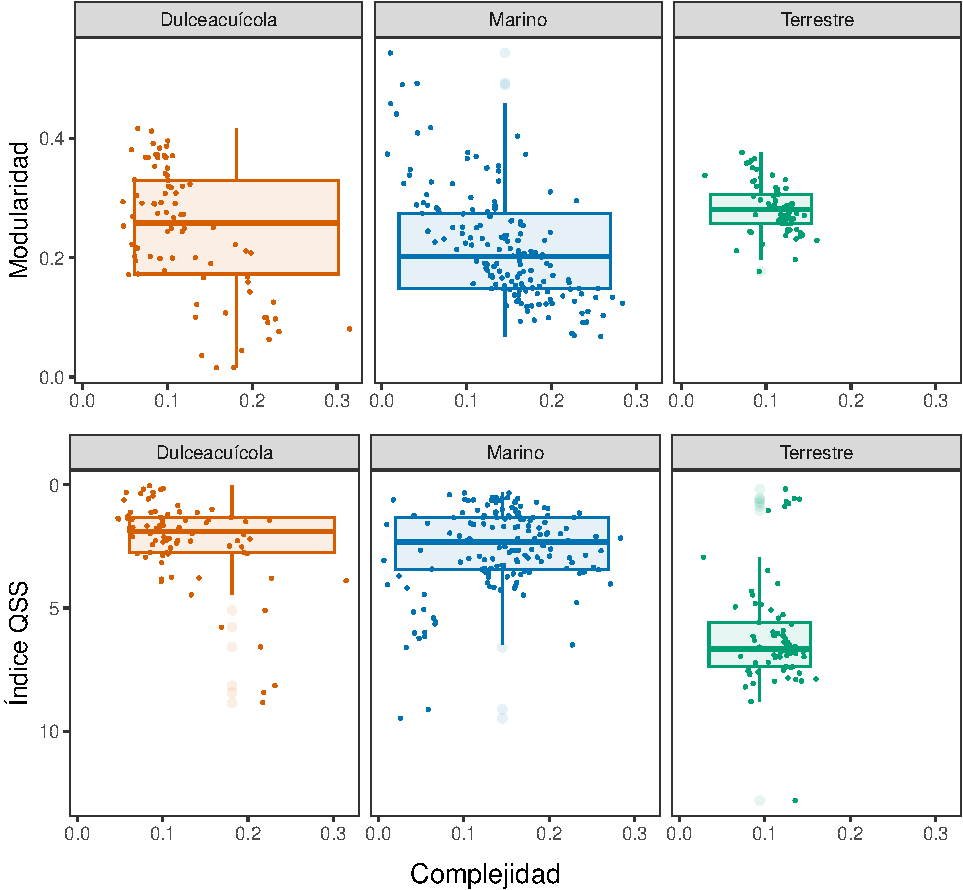
\includegraphics{MS_formateado_files/figure-latex/fig2-1} 

}

\caption{Modularidad e índice QSS según el tipo de ecosistema. Cada punto representa una red trófica. En el diagrama de cajas y bigotes, la altura de la caja representa el intercuartil 25-75, la línea horizontal la mediana y las líneas verticales superior e inferior los percentiles 95 y 5, respectivamente.}\label{fig:fig2}
\end{figure}

\newpage
\begin{figure}

{\centering \includegraphics{MS_formateado_files/figure-latex/fig3-1} 

}

\caption{Relación entre complejidad y (A) modularidad e (B) índice QSS en redes tróficas empíricas. Cada punto representa una red trófica. Regresión lineal para modularidad ($y = 0.40 - 1.2x, R^2 = 0.50, p-value < 2.16e-16$) e índice QSS ($y = 3.86 - 4.2x, R^2 < 0.01, p-value = 0.09$). En (B) la relación complejidad-QSS se muestran las regresiones de cuantiles 25 y 75.}\label{fig:fig3}
\end{figure}

\newpage
\begin{figure}

{\centering \includegraphics{MS_formateado_files/figure-latex/fig4-1} 

}

\caption{Relación complejidad-modularidad (panel superior) y complejidad-índice QSS (panel inferior) en redes tróficas empíricas según el tipo de ecosistema. Regresión lineal para redes dulceacuícolas (modularidad: $y = 0.4 - 1.3x, R^2 = 0.44, p-value < 0.001$; QSS: $y = - 0.13 - 18x, R^2 = 0.32, p-value < 0.001$), marinas (modularidad: $y = 0.38 - 1.1x, R^2 = 0.52, p-value < 0.001$; QSS: $y = - 3.5 - 6.8x, R^2 = 0.06, p-value < 0.002$) y terrestres (modularidad: $0.38 - 0.88x, R^2 = 0.24, p-value < 0.001$; QSS: $y = - 5.7 - 3x, R^2 < 0.01, p-value < 0.799$).}\label{fig:fig4}
\end{figure}

\hypertarget{literatura-citada}{%
\section*{Literatura Citada}\label{literatura-citada}}
\addcontentsline{toc}{section}{Literatura Citada}

\hypertarget{refs}{}
\begin{CSLReferences}{1}{0}
\leavevmode\vadjust pre{\hypertarget{ref-Allesina2008}{}}%
Allesina, S., \& Pascual, M. (2008). Network structure,
predator\textendash prey modules, and stability in large food webs.
\emph{Theoretical Ecology}, \emph{1}(1), 55--64.
\url{https://doi.org/10.1007/s12080-007-0007-8}

\leavevmode\vadjust pre{\hypertarget{ref-Allesina2015}{}}%
Allesina, S., \& Tang, S. (2015). The stability\textendash complexity
relationship at age 40: A random matrix perspective. \emph{Population
Ecology}, \emph{57}(1), 63--75.
\url{https://doi.org/10.1007/s10144-014-0471-0}

\leavevmode\vadjust pre{\hypertarget{ref-Blanchette2014}{}}%
Blanchette, M. L., Davis, A. M., Jardine, T. D., \& Pearson, R. G.
(2014). Omnivory and opportunism characterize food webs in a large
dry-tropics river system. \emph{Freshwater Science}, \emph{33}(1),
142--158. \url{https://doi.org/10.1086/674632}

\leavevmode\vadjust pre{\hypertarget{ref-Briand1987}{}}%
Briand, F., \& Cohen, J. (1987). \emph{Environmental {Correlates} of
{Food Chain Length} \textbar{} {Science}}.
https://www.science.org/doi/abs/10.1126/science.3672136.

\leavevmode\vadjust pre{\hypertarget{ref-Brose2019}{}}%
Brose, U., Archambault, P., Barnes, A. D., Bersier, L.-F., Boy, T.,
Canning-Clode, J., Conti, E., Dias, M., Digel, C., Dissanayake, A.,
Flores, A. A. V., Fussmann, K., Gauzens, B., Gray, C., Häussler, J.,
Hirt, M. R., Jacob, U., Jochum, M., Kéfi, S., \ldots{} Iles, A. C.
(2019). Predator traits determine food-web architecture across
ecosystems. \emph{Nature Ecology \& Evolution}, \emph{3}(6), 919--927.
\url{https://doi.org/10.1038/s41559-019-0899-x}

\leavevmode\vadjust pre{\hypertarget{ref-Brose2018}{}}%
Brose, U., \& et. al. (2018). \emph{{GlobAL daTabasE} of traits and food
{Web Architecture} ({GATEWAy}) v.1.0.} {iDiv Data Repository}.

\leavevmode\vadjust pre{\hypertarget{ref-Cebrian2004a}{}}%
Cebrian, J. (2004). Role of first-order consumers in ecosystem carbon
flow. \emph{Ecology Letters}, \emph{7}(3), 232--240.
\url{https://doi.org/10.1111/j.1461-0248.2004.00574.x}

\leavevmode\vadjust pre{\hypertarget{ref-Cebrian2004}{}}%
Cebrian, J., \& Lartigue, J. (2004). Patterns of {Herbivory} and
{Decomposition} in {Aquatic} and {Terrestrial Ecosystems}.
\emph{Ecological Monographs}, \emph{74}(2), 237--259.
\url{https://doi.org/10.1890/03-4019}

\leavevmode\vadjust pre{\hypertarget{ref-Cohen1978}{}}%
Cohen, J. E., \& Stephens, D. W. (1978). \emph{Food {Webs} and {Niche
Space}}. {Princeton University Press}.

\leavevmode\vadjust pre{\hypertarget{ref-Csardi2006}{}}%
Csardi, \& Nepusz. (2006). \emph{The igraph software package for complex
network research}.

\leavevmode\vadjust pre{\hypertarget{ref-Digel2014}{}}%
Digel, C., Curtsdotter, A., Riede, J., Klarner, B., \& Brose, U. (2014).
Unravelling the complex structure of forest soil food webs: Higher
omnivory and more trophic levels. \emph{Oikos}, \emph{123}(10),
1157--1172. \url{https://doi.org/10.1111/oik.00865}

\leavevmode\vadjust pre{\hypertarget{ref-Dodge2008}{}}%
Dodge, Y. (2008). Kruskal-wallis test. In \emph{The concise encyclopedia
of statistics} (pp. 288--290). {Springer New York}.

\leavevmode\vadjust pre{\hypertarget{ref-Dominguez-Garcia2019}{}}%
Domínguez-García, V., Dakos, V., \& Kéfi, S. (2019). Unveiling
dimensions of stability in complex ecological networks.
\emph{Proceedings of the National Academy of Sciences}, \emph{116}(51),
25714--25720. \url{https://doi.org/10.1073/pnas.1904470116}

\leavevmode\vadjust pre{\hypertarget{ref-Donohue2016}{}}%
Donohue, I., Hillebrand, H., Montoya, J. M., Petchey, O. L., Pimm, S.
L., Fowler, M. S., Healy, K., Jackson, A. L., Lurgi, M., McClean, D.,
O'Connor, N. E., O'Gorman, E. J., \& Yang, Q. (2016). Navigating the
complexity of ecological stability. \emph{Ecology Letters},
\emph{19}(9), 1172--1185. \url{https://doi.org/10.1111/ele.12648}

\leavevmode\vadjust pre{\hypertarget{ref-Dunne2009}{}}%
Dunne, J. A., \& Williams, R. J. (2009). Cascading extinctions and
community collapse in model food webs. \emph{Philosophical Transactions
of the Royal Society B: Biological Sciences}, \emph{364}(1524),
1711--1723. \url{https://doi.org/10.1098/rstb.2008.0219}

\leavevmode\vadjust pre{\hypertarget{ref-Dunne2002a}{}}%
Dunne, J. A., Williams, R. J., \& Martinez, N. D. (2002). Food-web
structure and network theory: {The} role of connectance and size.
\emph{Proceedings of the National Academy of Sciences}, \emph{99}(20),
12917--12922. \url{https://doi.org/10.1073/pnas.192407699}

\leavevmode\vadjust pre{\hypertarget{ref-Frelat2022}{}}%
Frelat, R., Kortsch, S., Kröncke, I., Neumann, H., Nordström, M. C.,
Olivier, P. E. N., \& Sell, A. F. (2022). Food web structure and
community composition: A comparison across space and time in the {North
Sea}. \emph{Ecography}, \emph{2022}(2).
\url{https://doi.org/10.1111/ecog.05945}

\leavevmode\vadjust pre{\hypertarget{ref-Gilbert2009}{}}%
Gilbert, A. J. (2009). Connectance indicates the robustness of food webs
when subjected to species loss. \emph{Ecological Indicators},
\emph{9}(1), 72--80. \url{https://doi.org/10.1016/j.ecolind.2008.01.010}

\leavevmode\vadjust pre{\hypertarget{ref-Grilli2016}{}}%
Grilli, J., Rogers, T., \& Allesina, S. (2016). Modularity and stability
in ecological communities. \emph{Nature Communications}, \emph{7}(1),
12031. \url{https://doi.org/10.1038/ncomms12031}

\leavevmode\vadjust pre{\hypertarget{ref-Guimera2005}{}}%
Guimerà, R., \& Nunes Amaral, L. A. (2005). Functional cartography of
complex metabolic networks. \emph{Nature}, \emph{433}(7028), 895--900.
\url{https://doi.org/10.1038/nature03288}

\leavevmode\vadjust pre{\hypertarget{ref-Jacquet2016}{}}%
Jacquet, C., Moritz, C., Morissette, L., Legagneux, P., Massol, F.,
Archambault, P., \& Gravel, D. (2016). No
complexity\textendash stability relationship in empirical ecosystems.
\emph{Nature Communications}, \emph{7}(1), 12573.
\url{https://doi.org/10.1038/ncomms12573}

\leavevmode\vadjust pre{\hypertarget{ref-King2018}{}}%
King, B. M., Rosopa, P. J., \& Minium, E. W. (2018). \emph{Statistical
{Reasoning} in the {Behavioral Sciences}}. {John Wiley \& Sons}.

\leavevmode\vadjust pre{\hypertarget{ref-Kortsch2015}{}}%
Kortsch, S., Primicerio, R., Fossheim, M., Dolgov, A. V., \& Aschan, M.
(2015). Climate change alters the structure of arctic marine food webs
due to poleward shifts of boreal generalists. \emph{Proceedings of the
Royal Society B: Biological Sciences}, \emph{282}(1814), 20151546.
\url{https://doi.org/10.1098/rspb.2015.1546}

\leavevmode\vadjust pre{\hypertarget{ref-Krause2003}{}}%
Krause, A. E., Frank, K. A., Mason, D. M., Ulanowicz, R. E., \& Taylor,
W. W. (2003). Compartments revealed in food-web structure.
\emph{Nature}, \emph{426}(6964), 282--285.
\url{https://doi.org/10.1038/nature02115}

\leavevmode\vadjust pre{\hypertarget{ref-Landi2018a}{}}%
Landi, P., Minoarivelo, H. O., Brännström, Å., Hui, C., \& Dieckmann, U.
(2018). Complexity and stability of ecological networks: A review of the
theory. \emph{Population Ecology}, \emph{60}(4), 319--345.
\url{https://doi.org/10.1007/s10144-018-0628-3}

\leavevmode\vadjust pre{\hypertarget{ref-Lenth2022}{}}%
Lenth, R. V. (2022). \emph{Emmeans: {Estimated Marginal Means}, aka
{Least-Squares Means}}.

\leavevmode\vadjust pre{\hypertarget{ref-Marina2018a}{}}%
Marina, T. I., Saravia, L. A., Cordone, G., Salinas, V., Doyle, S. R.,
\& Momo, F. R. (2018). Architecture of marine food webs: {To} be or not
be a {``small-world.''} \emph{PLOS ONE}, \emph{13}(5), e0198217.
\url{https://doi.org/10.1371/journal.pone.0198217}

\leavevmode\vadjust pre{\hypertarget{ref-Martinez1992}{}}%
Martinez, N. D. (1992). Constant {Connectance} in {Community Food Webs}.
\emph{The American Naturalist}, \emph{139}(6), 1208--1218.
\url{https://doi.org/10.1086/285382}

\leavevmode\vadjust pre{\hypertarget{ref-May1973}{}}%
May, R. (1973). \emph{Stability and complexity in model ecosystems}.
{Princeton University Press}.

\leavevmode\vadjust pre{\hypertarget{ref-McCann2000}{}}%
McCann, K. S. (2000). The diversity\textendash stability debate.
\emph{Nature}, \emph{405}(6783), 228--233.
\url{https://doi.org/10.1038/35012234}

\leavevmode\vadjust pre{\hypertarget{ref-Montoya2003a}{}}%
Montoya, J. M., Rodríguez, M. A., \& Hawkins, B. A. (2003). Food web
complexity and higher-level ecosystem services. \emph{Ecology Letters},
\emph{6}(7), 587--593.
\url{https://doi.org/10.1046/j.1461-0248.2003.00469.x}

\leavevmode\vadjust pre{\hypertarget{ref-Mougi2022}{}}%
Mougi, A. (2022). Predator interference and
complexity\textendash stability in food webs. \emph{Scientific Reports},
\emph{12}(1), 2464. \url{https://doi.org/10.1038/s41598-022-06524-w}

\leavevmode\vadjust pre{\hypertarget{ref-Naeem1997}{}}%
Naeem, S., \& Li, S. (1997). Biodiversity enhances ecosystem
reliability. \emph{Nature}, \emph{390}(6659), 507--509.
\url{https://doi.org/10.1038/37348}

\leavevmode\vadjust pre{\hypertarget{ref-Namba2015}{}}%
Namba, T. (2015). Multi-faceted approaches toward unravelling complex
ecological networks. \emph{Population Ecology}, \emph{57}(1), 3--19.
\url{https://doi.org/10.1007/s10144-015-0482-5}

\leavevmode\vadjust pre{\hypertarget{ref-Nowlin2008}{}}%
Nowlin, W. H., Vanni, M. J., \& Yang, L. H. (2008). Comparing {Resource
Pulses} in {Aquatic} and {Terrestrial Ecosystems}. \emph{Ecology},
\emph{89}(3), 647--659. \url{https://doi.org/10.1890/07-0303.1}

\leavevmode\vadjust pre{\hypertarget{ref-Pace2004}{}}%
Pace, M. L., Cole, J. J., Carpenter, S. R., Kitchell, J. F., Hodgson, J.
R., Van de Bogert, M. C., Bade, D. L., Kritzberg, E. S., \& Bastviken,
D. (2004). Whole-lake carbon-13 additions reveal terrestrial support of
aquatic food webs. \emph{Nature}, \emph{427}(6971), 240--243.
\url{https://doi.org/10.1038/nature02227}

\leavevmode\vadjust pre{\hypertarget{ref-Paine1966}{}}%
Paine, R. T. (1966). Food {Web Complexity} and {Species Diversity}.
\emph{The American Naturalist}, \emph{100}(910), 65--75.
\url{https://doi.org/10.1086/282400}

\leavevmode\vadjust pre{\hypertarget{ref-Pascual2005}{}}%
Pascual, M., \& Dunne, J. A. (2005). \emph{Ecological {Networks}:
{Linking Structure} to {Dynamics} in {Food Webs}}. {Oxford University
Press}.

\leavevmode\vadjust pre{\hypertarget{ref-Perkins2022}{}}%
Perkins, D. M., Hatton, I. A., Gauzens, B., Barnes, A. D., Ott, D.,
Rosenbaum, B., Vinagre, C., \& Brose, U. (2022). Consistent
predator-prey biomass scaling in complex food webs. \emph{Nature
Communications}, \emph{13}(1), 4990.
\url{https://doi.org/10.1038/s41467-022-32578-5}

\leavevmode\vadjust pre{\hypertarget{ref-Rodriguez2022}{}}%
Rodriguez, I. D., Marina, T. I., Schloss, I. R., \& Saravia, L. A.
(2022). Marine food webs are more complex but less stable in
sub-{Antarctic} ({Beagle Channel}, {Argentina}) than in {Antarctic}
({Potter Cove}, {Antarctic Peninsula}) regions. \emph{Marine
Environmental Research}, \emph{174}, 105561.
\url{https://doi.org/10.1016/j.marenvres.2022.105561}

\leavevmode\vadjust pre{\hypertarget{ref-Rodriguez-Florez2023}{}}%
Rodríguez-Flórez, C. N., Paczkowska, J., Martín, J., Gil, M. N.,
Flores-Melo, X., \& Malits, A. (2023). Terrigenous dissolved organic
matter input and nutrient-light-limited conditions on the winter
microbial food web of the {Beagle Channel}. \emph{Journal of Marine
Systems}, 103860. \url{https://doi.org/10.1016/j.jmarsys.2023.103860}

\leavevmode\vadjust pre{\hypertarget{ref-Saravia2022a}{}}%
Saravia, L. A. (2022). \emph{Multiweb: {Ecological} network analyses
including multiplex networks}.

\leavevmode\vadjust pre{\hypertarget{ref-Shurin2005}{}}%
Shurin, J. B., Gruner, D. S., \& Hillebrand, H. (2005). All wet or dried
up? {Real} differences between aquatic and terrestrial food webs.
\emph{Proceedings of the Royal Society B: Biological Sciences},
\emph{273}(1582), 1--9. \url{https://doi.org/10.1098/rspb.2005.3377}

\leavevmode\vadjust pre{\hypertarget{ref-Stouffer2011}{}}%
Stouffer, D. B., \& Bascompte, J. (2011). Compartmentalization increases
food-web persistence. \emph{Proceedings of the National Academy of
Sciences}, \emph{108}(9), 3648--3652.
\url{https://doi.org/10.1073/pnas.1014353108}

\leavevmode\vadjust pre{\hypertarget{ref-RCoreTeam2022}{}}%
Team, R. C. (2022). \emph{R: {A Language} and {Environment} for
{Statistical Computing}}. R Foundation for Statistical Computing.

\leavevmode\vadjust pre{\hypertarget{ref-Thompson2012}{}}%
Thompson, R. M., Dunne, J. A., \& Woodward, G. (2012). Freshwater food
webs: Towards a more fundamental understanding of biodiversity and
community dynamics. \emph{Freshwater Biology}, \emph{57}(7), 1329--1341.
\url{https://doi.org/10.1111/j.1365-2427.2012.02808.x}

\leavevmode\vadjust pre{\hypertarget{ref-Thompson2007}{}}%
Thompson, R. M., Hemberg, M., Starzomski, B. M., \& Shurin, J. B.
(2007). Trophic {Levels} and {Trophic Tangles}: {The Prevalence} of
{Omnivory} in {Real Food Webs}. \emph{Ecology}, \emph{88}(3), 612--617.
\url{https://doi.org/10.1890/05-1454}

\leavevmode\vadjust pre{\hypertarget{ref-Vargha2000}{}}%
Vargha, A., \& Delaney, H. D. (2000). A {Critique} and {Improvement} of
the {CL Common Language Effect Size Statistics} of {McGraw} and {Wong}.
\emph{Journal of Educational and Behavioral Statistics}, \emph{25}(2),
101--132. \url{https://doi.org/10.3102/10769986025002101}

\leavevmode\vadjust pre{\hypertarget{ref-Wickham2022}{}}%
Wickham, H., François, R., Henry, L., \& Müller, K. (2022). \emph{Dplyr:
{A Grammar} of {Data Manipulation}}.

\leavevmode\vadjust pre{\hypertarget{ref-Wilkinson1973}{}}%
Wilkinson, G. N., \& Rogers, C. E. (1973). Symbolic {Description} of
{Factorial Models} for {Analysis} of {Variance}. \emph{Journal of the
Royal Statistical Society. Series C (Applied Statistics)}, \emph{22}(3),
392--399. \url{https://doi.org/10.2307/2346786}

\leavevmode\vadjust pre{\hypertarget{ref-Windsor2023}{}}%
Windsor, F. M., van den Hoogen, J., Crowther, T. W., \& Evans, D. M.
(2023). Using ecological networks to answer questions in global
biogeography and ecology. \emph{Journal of Biogeography}, \emph{50}(1),
57--69. \url{https://doi.org/10.1111/jbi.14447}

\leavevmode\vadjust pre{\hypertarget{ref-Yletyinen2016}{}}%
Yletyinen, J., Bodin, Ö., Weigel, B., Nordström, M. C., Bonsdorff, E.,
\& Blenckner, T. (2016). Regime shifts in marine communities: A complex
systems perspective on food web dynamics. \emph{Proceedings of the Royal
Society B: Biological Sciences}, \emph{283}(1825), 20152569.
\url{https://doi.org/10.1098/rspb.2015.2569}

\leavevmode\vadjust pre{\hypertarget{ref-Yodzis1992}{}}%
Yodzis, P., \& Innes, S. (1992). Body {Size} and {Consumer-Resource
Dynamics}. \emph{The American Naturalist}, \emph{139}(6), 1151--1175.
\url{https://doi.org/10.1086/285380}

\end{CSLReferences}

\end{document}
